\chapter{Précédents dans la littérature}
\par A notre connaissance, il existe, dans la littérature, assez peu de modèles ayant pour but de quantifier objectivement le réalisme physiologique. Ce type de modèle ne doit pas être confondu avec les méthodes de qualification de la qualité de l'image qui elles sont basées sur une comparaison entre une image source et cette même image après qu'elle soit passée à travers tout un processus de transformation (comme par exemple, un encodage vidéo) \citep{cadik_human_2004, winkler_quality_2000} (voir Fig. \ref{fig:quality_process}). Actuellement, il existe déjà un grand nombre de méthodes pour la qualité d'image, notamment pour des images 2D (images statiques ou vidéos). Ces dernières années, l'accent à plutôt été mis sur le développement de techniques de qualification de la qualité pour des images 3D. On peut trouver un certain nombre de revues de ces techniques dans la littérature \citep{moorthy_subjective_2013, moorthy_survey_2013} voire même avec une dimension subjective en plus \citep{beghdadi_survey_2013}.
	
	\begin{figure}[h]
		\centering
		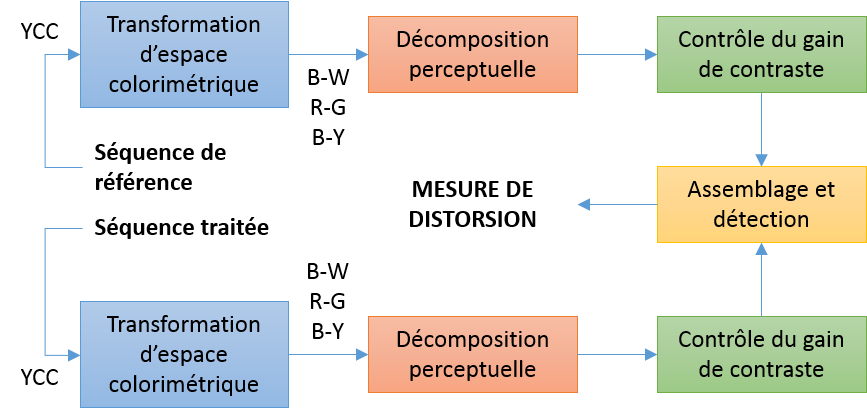
\includegraphics[scale=1]{Figures/ImageQualityWinkler}
		\caption{Fonctionnement du processus de mesure de qualité d'image pour des séquences vidéo 2D.}{Traduction d'une figure reprise de \cite{winkler_quality_2000}}
		\label{fig:quality_process}
	\end{figure}
	
	\par Le réalisme en tant que tel est quant à lui en général plutôt mesuré par une question directe sur le réalisme de l'expérience à laquelle le sujet vient de participer (ce qui est à relier avec la quatrième acceptation du réalisme, le réalisme \textit{psychologique} et non pas le réalisme \textit{physiologique}). Des approches plus détaillées peuvent se servir de questionnaires \citep{fucentese_evaluation_2015, fiard_initial_2014}.
	
	\par Néanmoins, on trouve quelques approches objectives pour la définition du réalisme bien que ce ne soit pas forcément leur objectif principal:	
		\begin{itemize}
			\item Le modèle de Rose \citep{rose_sensitivity_1948,burgess_rose_1999},
			\item Le modèle d'observateur idéal \citep{geisler_ideal_2003},
			\item Le tableau de Burdea et Coiffet \citep{burdea_realite_1993}.
		\end{itemize}
		
		\section{Modèle de Rose}		
		\par Le modèle de Rose est une première tentative (à l'époque pour la télévision en noir et blanc !) de caractérisation de "l'enregistreur d'image" idéal, vis à vis de la vision humaine. Le modèle est conçu pour la capture d'un objet unique, c'est à dire que le modèle donne les caractéristiques qu'un objet unique doit avoir pour être capturé par l'enregistreur idéal. On peut le décrire par l'équation  suivante (Eq. \ref{eq:modèle_rose}), avec $B$ la luminance de l'objet en footLamberts\footnote{NB: $1~fL \approx 3.426~cd/m^2$}, $C$ le contraste de l'objet comparé au background (en pourcentage) et $\alpha$ l'angle visuel sous lequel l'objet est vu par l'enregistreur.
		
		\begin{equation}
			BC^2\alpha^2 = \text{constante}
			\label{eq:modèle_rose} 
		\end{equation}
		
		\section{Observateur idéal \& théorie de détection du signal}		
		\par La définition d'un <<~observateur idéal~>> est basée sur une théorie appelée <<~détection du signal~>> (Signal Detection Theory). Cette théorie décrit la capabilité d'un système à discerner un pattern spécifique au milieu d'autres patterns ou bien au milieu d'un bruit (voir Fig. \ref{fig:signal_detection_theory}). Le théorie de détection du signal est également basée sur la théorie bayésienne qui est l'interprétation du concept de probabilités comme état de savoir -la forme est visible ou non- plutôt qu'une fréquence ou une propension d'apparition d'un phénomène. La théorie de détection du signal inclut également des probabilités de détection et des seuils de vision. Cependant, les observateurs idéaux sont utilisés pour une unique tâche bien spécifique (au contraire de la vision qui se veut généraliste) telle que la détection de photon, la détection de forme, l'identification ...
		
		\begin{figure}[h]
			\centering
			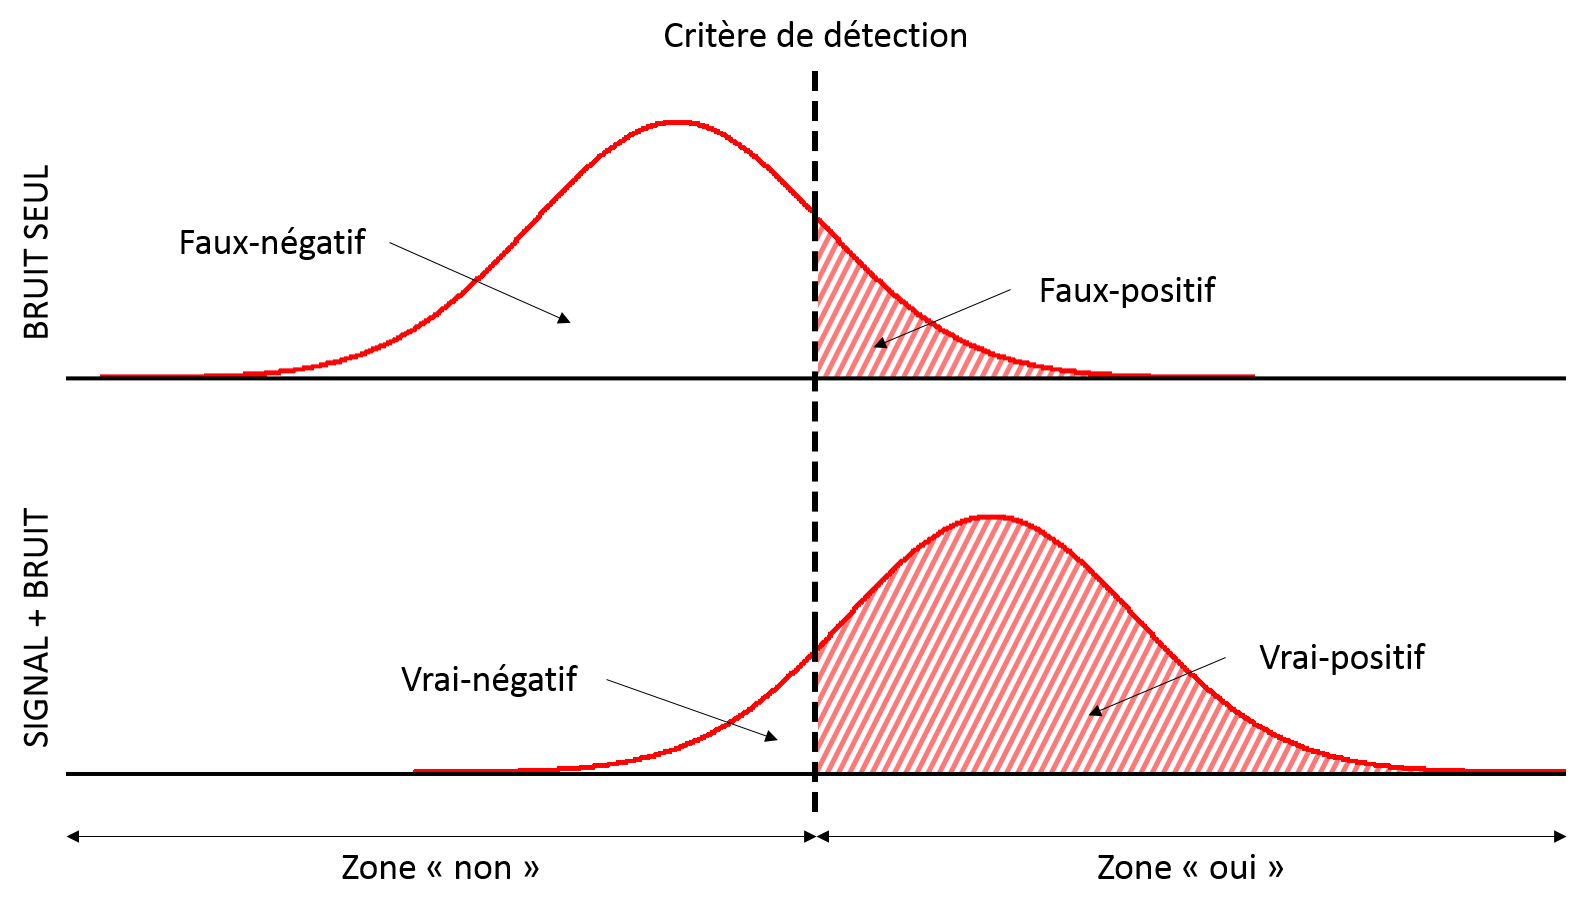
\includegraphics[scale=.5]{Figures/SignalDetectionTheory}
			\caption{Illustration de la théorie de détection du signal. Répartition des probabilités de détection autour d'un seuil de détection déterminé (critère de détection)}
			\label{fig:signal_detection_theory}
		\end{figure}
		
		\section{Tableau de Burdea \& Coiffet}
		\par La démarche de Burdea et Coiffet est celle qui se rapproche le plus de la nôtre. On a vu précédemment qu'ils considèrent que le système de Réalité Virtuelle, par construction, implique l'intégralité des sens de l'homme. Ils notent également, qu'en dépit du risque de difficulté, <<~il apparait hautement nécessaire d'évaluer ou de qualifier les systèmes de RV~>>. Ils vont même plus loin en <<~[se demandant] si les outils et les simulations de RV s'adressent correctement à l'homme, c'est à dire s'adressent conformément à ses habitudes de stimulation~>> \citep{burdea_realite_1993}.
		
		\par Burdea et Coiffet posent plusieurs définitions nécessaire à l'évaluation des systèmes de Réalité Virtuelle:
		\begin{itemize}
			\item La reproduction sensorielle est la combinaison de l'excitation des récepteurs mais également de la contextualisation de cette excitation: le stimulus doit être cohérent avec les autres sens et la situation.
			\item L'évaluation est l'action de déterminer les qualifications du contrôle et de mesurer le respect de ces qualifications par le système.
			\item Le contrôle est l'interprétation par l'homme des informations qui s'adressent à ses sens.
		\end{itemize}
		
		\par Les auteurs mettent en avant la difficulté de séparation entre les qualités du système et celles de l'application. Ils proposent néanmoins trois grandes catégories de paramètres caractérisants la vision totale (voir Fig. \ref{fig:burdea_coiffet_tableau}). Ces dernières sont: les conditions ergonomiques générales, les conditions physiologiques de vision et les conditions psychologiques de vision. On s'intéresse tout particulièrement à la deuxième catégorie, qui se décompose en sept paramètres:
		\begin{itemize}
			\item l'amplitude du champ de vision,
			\item la fréquence de rafraichissement,
			\item le respect de la convergence du regard,
			\item la résolution spatiale de l'image,
			\item le niveau d'éclairement et de luminosité adapté à l'œil,
			\item la perception du relief,
			\item la discrimination des couleurs.
		\end{itemize}
		
	\begin{figure}[h]
		\centering
		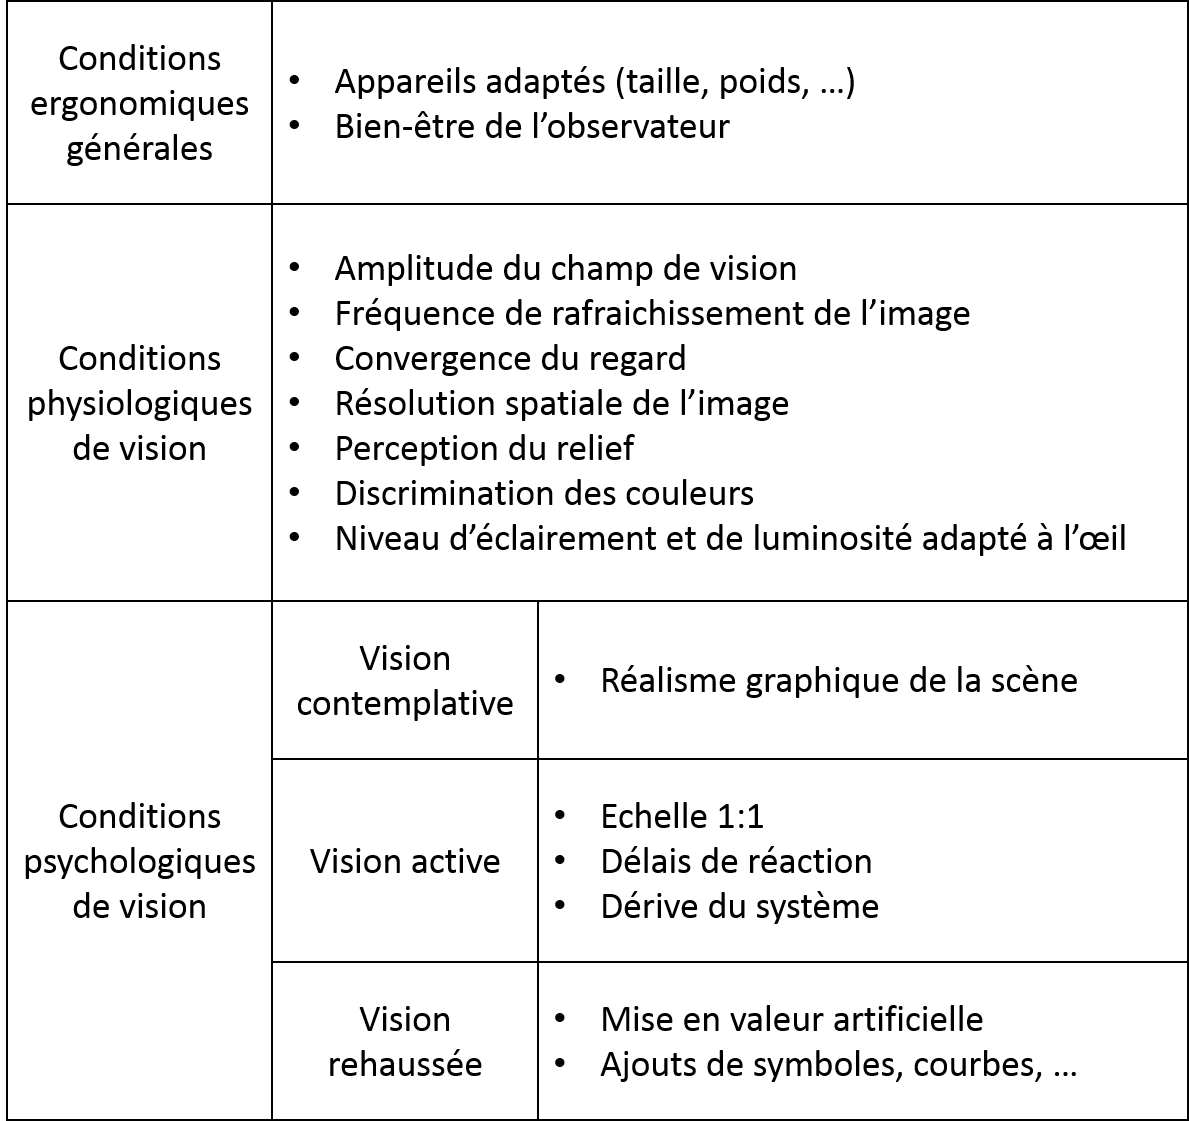
\includegraphics[scale=.75]{Figures/BurdeaCoiffetTableau}
		\caption{Paramètres caractérisant la vision totale}{Figure reproduite de \citep{burdea_realite_1993}}
		\label{fig:burdea_coiffet_tableau}
	\end{figure}
	
	\par Si Burdea et Coiffet pointent un certain nombre de paramètres qu'ils convient de mesurer pour estimer la qualité de la reproduction sensorielle, ils restent néanmoins assez limités sur les valeurs à atteindre.
	
	\par Pour la fréquence de rafraichissement de l'image ils semblent considérer qu'une valeur entre 14 et 30 soit suffisante: à partir de 25 à 30 images par seconde, l'œil est parfaitement abusé, et on observe de forte dégradations de la performance en téléopération en dessous de 14 images par seconde.
	
	\par Pour la perception du relief, ils se limitent à avancer que celle-ci résulte de la stéréo, bien qu'il existe aussi des indices monoscopiques.
	
	\par Ils rappellent ensuite que la discrimination des couleurs est basée sur la discrimination visuelle qui englobe l'acuité visuelle, l'acuité de reconnaissance, l'acuité de détection et l'acuité de résolution. Toutes ces acuités sont influencées par la luminance, le contraste, la durée d'observation, le rapport de luminance dans la scène, le mouvement de la cible et l'éblouissement. De même, si l'œil humain peut voir plusieurs millions de couleurs, il ne peut, toujours selon ces auteurs, en voir que 8 à la fois.
	
	\par Enfin, les auteurs mettent en avant la nécessité d'une faible latence, que ce soit pour la vision contemplative (le mouvement de l'environnement doit être synchronisé avec le mouvement de la tête) ou pour la réactivité du système qui doit être aux alentours des temps de réaction de l'homme, que les auteurs estiment autour de 0.1 seconde, soit $100~ms$.
	
	\chapter{Score de réalisme}
	\section{Ambition}	
	\par On a vu dans les modèles présentés précédemment dans l'introduction, et notamment dans celui de Rose qui mêle dans une équation mathématique simple des grandeurs essentielles pour le réalisme (contraste, luminance, taille), une approche pragmatique de la définition du réalisme physiologique. Néanmoins, il manque toujours une dimension à ces modèles: les modèles de Rose et d'observateur idéal prédisent pour l'un les qualités optimales d'affichage et pour l'autre le moment à partir duquel l'œil humain va percevoir l'objet puis une description de la probabilité de plus en plus élevée de le percevoir, mais jamais les deux en même temps.
	
	\par Au delà de ces modèles, on souhaite être capable de pouvoir quantifier le biais qu'il existe entre ce qui est affiché dans un environnement virtuel et la qualité de perception de l'utilisateur. C'est à dire non seulement être capable de dire quelles sont les conditions optimales pour que le système visuel humain interagisse avec l'affichage immersif mais aussi pouvoir apprécier les conditions non-optimales, tel le système de probabilité dans le modèle d'observateur idéal. On souhaite néanmoins réfléchir à une autre approche que celle probabiliste pour se rapprocher d'une démarche plus pragmatique.
	
	\par Cette méthode pourrait alors indiquer à quel point l'interaction entre le système visuel humain et l'affichage est différente de l'interaction qui aurait lieu dans le monde naturel et ce de manière tangible, mesurée. Pour que l'évaluation soit fiable et répétable, la quantification doit être objective et doit dépendre de critères physiques du système d'affichage (hardware).
	
	\par On propose alors une évaluation de la performance d'un système via un score qui dépeindrait, pour un système immersif donné et pour une situation donnée, à quel point le simulateur est efficace pour transmettre le bon niveau d'informations visuelles et, étant dans un système de Réalité Virtuelle, le bon niveau d'indices d'immersion. De manière analogue à ce que proposent Burdea et Coiffet pour leurs critères physiologiques de vision, notre score ne doit pas dépendre de critères propres à l'environnement 3D et garder ainsi son indépendance vis à vis de la qualité de ce qui est affiché. Les logiciels utilisés peuvent évidemment avoir un impact sur les critères du modèle (la nombre d'images par seconde ou la latence par exemple). On fait donc l'hypothèse, pour l'ensemble des travaux, que la partie logicielle ne dégrade pas sensiblement les caractéristiques du système et que l'on travaille bien sur la performance maximale atteignable par ce dernier.
	
	\begin{figure}[h]
		\centering
		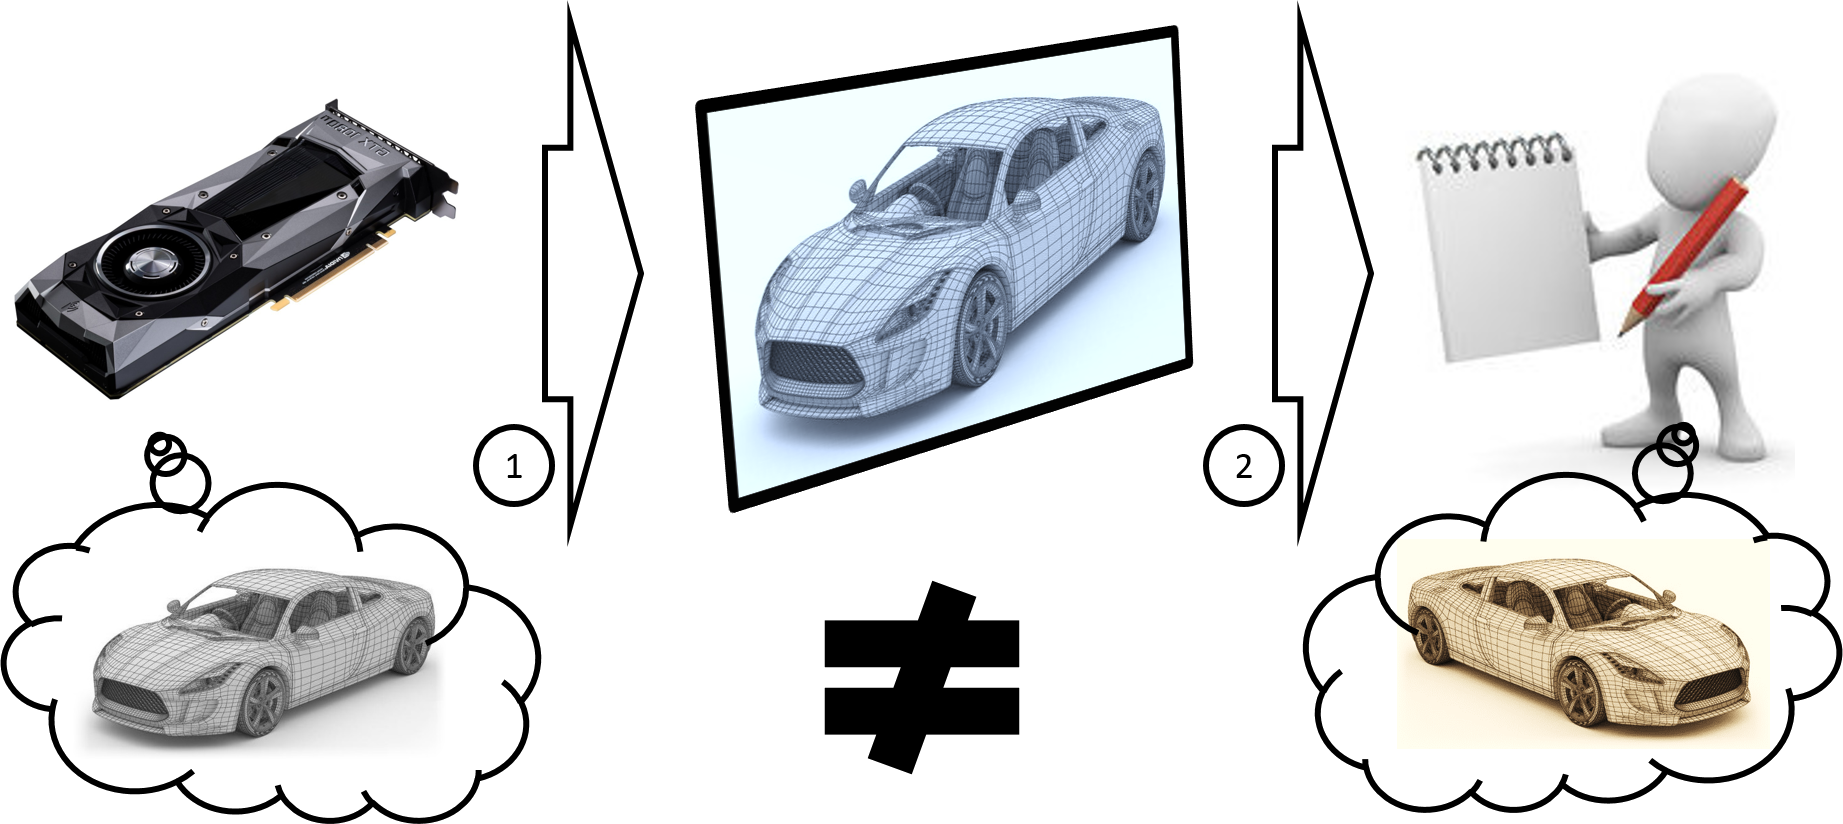
\includegraphics[scale=.45]{Figures/ImageBias}
		\caption{Illustration de la différence qu'il existe entre les consignes données par la carte graphique (1) et les informations visuelles reçues par l'observateur (2).}
		\label{fig:image_bias}
	\end{figure}
			
	\section{Méthodologie}
	\par On propose donc un système de score qui serait basé sur le système visuel humain. Ce score est en fait la réunion d'un certain nombre de sous-scores chacun lié à une caractéristique de la vision et/ou de l'immersion dépendante de la vision (c'est à dire les critères immersifs dérivés directement du système visuel ou du système en lui même). Chaque critère est jugé indépendamment puis contribue à la note globale via une pondération.
	
	\par La première étape était donc logiquement d'avoir une connaissance et une compréhension approfondie du système visuel humain. Comme on a pu voir dans la première partie, qui présente cette étude de l'état de l'art, on s'est intéressé d'abord au fonctionnement de l'œil en lui-même puis de ce qu'il se passe après, que ce soit le traitement nerveux ou le traitement par le cerveau. L'accent a ensuite été mis sur le contraste et la couleur qui sont deux des grandes caractéristiques de l'image ainsi que la perception visuelle de la profondeur. Enfin, certaines influences, classées ici abusivement comme << physiologiques >>, modifient le processus normal de la vision et doivent être, si possible, prises en compte.
	
	\par Ensuite, une fois cette connaissance acquise il a fallu découper le processus de vision et les facteurs d'immersions en différents critères. Ce processus a été long et compliqué, et fait l'objet d'un chapitre pour le détailler (voir par la suite). Ces critères se veulent indépendants les uns des autres mais des relations ont quand même parfois été relevées entre certains critères. Par exemple, la précision de la vision dépend dans certains cas de la luminosité: une situation bien éclairée permet de voir bien plus précisément qu'une situation mal éclairée. Pour plus de simplicité et de clarté, on a regroupé les critères par domaine.
	
	\par Troisièmement, une fois les critères établis, il convient de les évaluer. Pour ce faire, on propose d'attribuer une note comprise entre 0 et 100 à chacun des critères du modèle. Cette note modélise le fonctionnement du critère en question: la note de 0 représente les conditions dans lesquelles le système de vision n'est pas capable d'utiliser le mécanisme (ou peut l'utiliser mais n'en tire aucune information utile) tandis que la note de 100 représente le fonctionnement ou la performance maximal-e du mécanisme de vision. On rajoute également une note intermédiaire à 80 qui représente le fonctionnement nominal du mécanisme de vision. La valeur de 80 est plus probablement la valeur de score à viser car la valeur de 100 représente le maximum possible de l'œil humain et pourrait être considéré comme de la sur-qualité par rapport à la performance nominale. Il est évident que dans certaines applications, atteindre la valeur de 100 peut être une nécessité. Cette démarche est confortée par le fait que la Commission Internationale pour l'Eclairage (CIE) procède de la même manière (noter sur une valeur de 100 en adjugeant 80 à la valeur nominale) dans son modèle de performance visuelle en fonction de la luminosité et du contraste (que l'on abordera plus loin dans le manuscrit).
	
	\par La notation en elle même est, principalement basée sur la littérature: on cherche les valeurs correspondants aux fonctionnements minimal, nominal et maximal. On cherche ensuite une loi mathématique simple permettant de décrire l'évolution de la note en fonction des valeurs clefs du mécanisme visuel. Si on a pu appliquer cette méthode pour la majorité des cas, certains critères ne se prêtent pas à un tel traitement et ont bénéficié d'une notation particulière. Cette notation sera explicitée plus bas, au cas par cas, dans la présentation des critères retenus dans la dernière version du modèle.
	
	\begin{figure}[h]
		\centering
		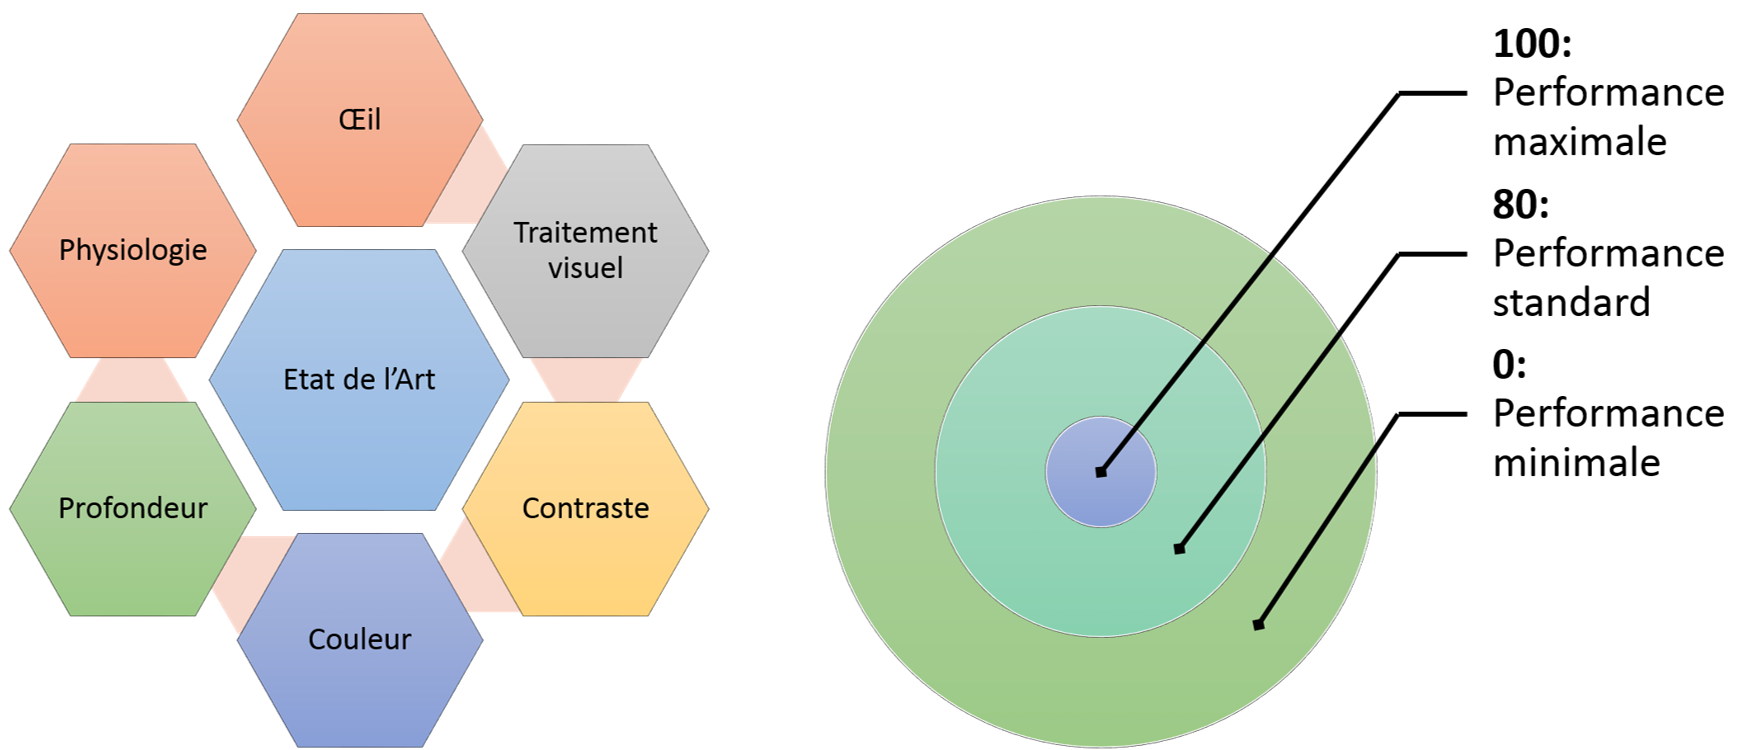
\includegraphics[scale=.50]{Figures/EDLAProcessScoreTarget}
		\caption{Résumé des étapes d'état de l'art pour la construction du modèle et répartition des objectifs de représentation des notes intermédiaires dans le score de réalisme.}
		\label{fig:edla_process_score_target}
	\end{figure}
	
	\chapter{Proposition de modèle}
	\par Pour faciliter la lecture et la compréhension du chapitre, on propose d'expliquer sommairement ici certaines distinctions entre des termes proches qui seront utilisés. Tous ces termes seront explicités en détail par la suite dans les deux prochains chapitres.

	\par L' << acuité monoscopique >>, aussi connue sous le nom d'acuité visuelle est définie par le Vulgaris Médical\footnote{Acuité visuelle. Dans \textit{Vulgaris Médical}. Consulté le 20/09/2017, http://www.vulgaris-medical.com/encyclopedie-medicale/acuite-visuelle (Lien court: https://lc.cx/GfSj)} de la sorte:
	\begin{quote}
		L'acuité visuelle est la capacité de discernement des informations apportées au cerveau par la vue. C'est la performance visuelle, elle mesure le pouvoir de l'œil à distinguer nettement les détails, avec et sans lunettes.
	\end{quote}
	Elle ne doit pas être confondue avec << l'acuité stéréoscopique >> qui est la capacité de l'œil à distinguer une très petite différence de profondeur à une distance donnée.
	
	\par De même, le << champ de vision >> est ce qu'un individu perçoit à un instant $t$ sans possibilité de bouger la tête ou l'œil dans son orbite. Le << champ de regard >> englobe tout ce qu'un individu peut voir en ayant le droit de bouger la tête et les yeux. Par définition, le champ de regard est donc plus grand que le champ de vision.
	
	\par Enfin, la gamme dynamique (Dynamic Range en anglais) est, dans le domaine de l'image, le rapport entre le minimum et le maximum de luminance atteignable. Il est définit par rapport à la courbe de gamma obtenue avec un écran cathodique. Le HDR (ou High Dynamic Range) représente un ratio entre le minimum et le maximum de luminance possible supérieur au ratio standard. HDR sous entend en général une technique d'imagerie pour augmenter artificiellement les extrema lumineux pendant la capture d'image.
	
	\section{Propositions préliminaires}
	\par Avant d'arriver à la modélisation finale du score (voir ci-après) nous sommes passés par un certain nombre de pistes et de modélisations. Nous allons présenter ici les différentes étapes qui ont vu le jour. Chacune des modélisations préliminaires amène un concept élémentaire qui sera utilisé pour faire notre proposition finale: l'inventaire, l'évaluation et la classification des critères du modèle.
	
	\subsection{Inventaire des critères visuels pour le réalisme}
	\par Initialement (Fig. \ref{fig:modèle_1}), la proposition était de faire un score simple qui réunirait les critères de base, accompagné d'un score avancé qui servirait à raffiner l'évaluation du système. La composition du modèle est basée sur les capacités de la vision que sont l'acuité, l'attention périphérique, la coordination des yeux, la perception de la profondeur, le focus et la perception des couleurs. Si le focus reste un problème insoluble en VR à cause du conflit accommodation-vergence toutes les autres capacités sont néanmoins traitables. Un critère répondant à la coordination des yeux n'est cependant pas encore proposé dans cette première modélisation. Le score simple est alors décliné selon les critères suivants:
	\begin{itemize}
		\item le contraste
		\item l'acuité monoscopique
		\item l'acuité stéréoscopique
		\item la latence
		\item le nombre d'images par seconde
		\item le respect de l'échelle 1:1
		\item la couverture du nombre de couleurs visibles
		\item la taille de l'HDR (ratio de luminance)
	\end{itemize}
	Tandis que le test avancé rajoute en plus du score simple qui reste toujours à effectuer:
	\begin{itemize}
		\item le champ de vision
		\item le champ de regard
		\item les maximum et minimum de luminance
	\end{itemize}
	Le tout étant rassemblé dans une équation de somme pondérée (Eq. \ref{eq:premiere_modelisation}), avec $\Sigma$ la valeur du score général du système, $\lambda_i$ la pondération du critère $i$, $\sigma_i$ la valeur observée du critère et $F_{100}$ la fonction donnant la note entre 0 et 100 du critère. 
	
	\begin{equation}
		\Sigma = \frac{1}{\sum_{i = 1}^{n} \lambda_i} \sum_{i = 1}^{n} \lambda_i F_{100,i}(\sigma_i)
		\label{eq:premiere_modelisation}
	\end{equation}
	
	\begin{figure}[h]
		\centering
		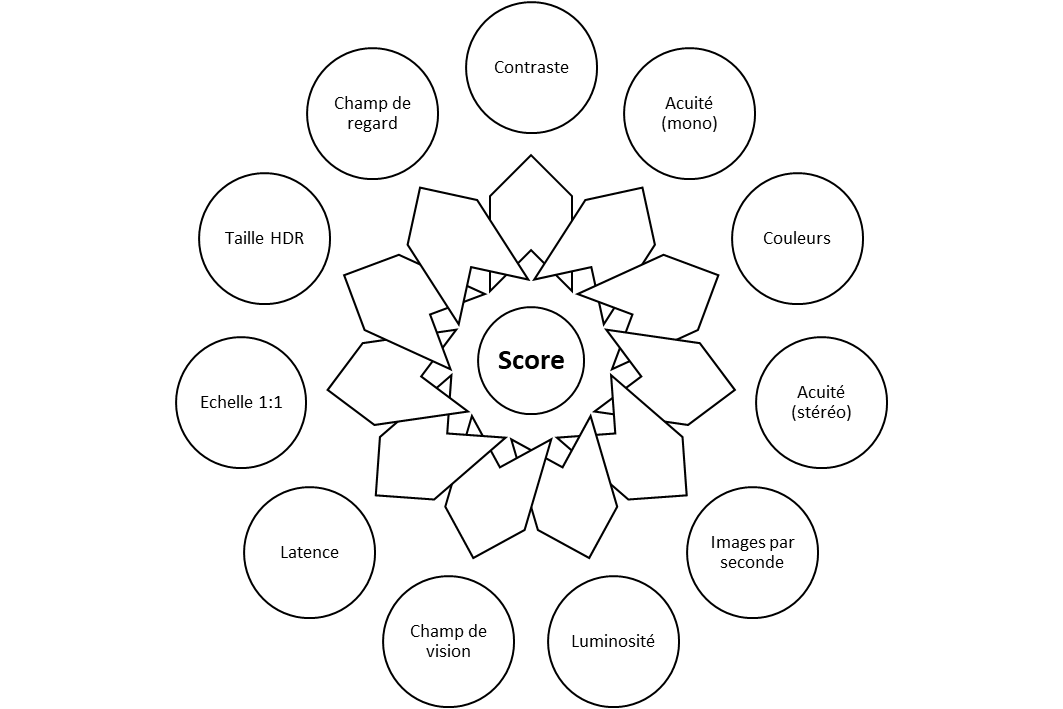
\includegraphics[scale=.8]{Figures/Modele1_2}
		\caption{Première modélisation du score de réalisme.}
		\label{fig:modèle_1}
	\end{figure}
	
	\subsection{Introduction de l'évaluation des critères}
	\par La seconde étape de la modélisation  (Fig. \ref{fig:modèle_2}) est assez proche de la première puisqu'on garde une liste quasiment similaire de critères de base : contraste, acuités monoscopique et stéréoscopique, images par seconde, couleur, luminosité et champ de vision. On retire le concept de score simple et de score avancé pour se concentrer sur un mélange des critères des deux scores précédemment envisagés en enlevant cependant les critères de champ de regard, de latence et d'échelle 1:1. Ces trois derniers facteurs, plus un critère d'uniformité, sont isolés dans une catégorie appelée << facteurs limitants >> et doivent interdire à la note globale de passer au delà d'un certain seuil en fonction de leur valeur. Ces facteurs sont de type booléens (au-dessus ou en-dessous d'un seuil): si le système propose une valeur moins bonne que celle demandée par le facteur limitant, la note globale maximale atteignable est automatiquement tronquée.
	
	\par Il était également envisagé de permettre un système de logique combinatoire entre les facteurs limitants. Par exemple, si le score de la latence est inférieur à 50 la note globale maximale atteignable est tronquée à 90 alors que si le score de la latence est inférieur à 60 et que le score de champ de regard est inférieur à 40 le score final maximal atteignable est diminué cette fois à 75.
	
	\par C'est à partir de cette modélisation qu'apparaissent les jalons spécifiques de performance: la note de 0 pour le minimum de performance possible ou acceptable, la note de 80 pour la performance standard du système visuel humain et la note de 100 pour sa performance maximale. Un jalon optionnel (en fonction de la littérature) à 60 pour une performance dite << acceptable >> a même été un temps envisagé avant d'être rejeté faute de pertinence et de répétabilité sur tous les critères.
	
	\begin{figure}[h]
		\centering
		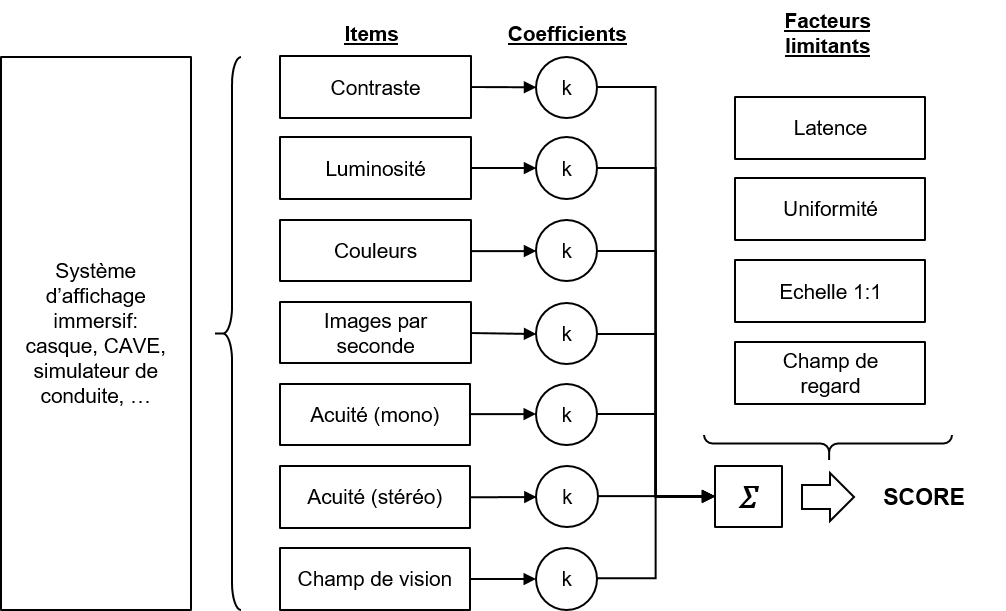
\includegraphics[scale=.8]{Figures/Modele2_2}
		\caption{Deuxième modélisation du score de réalisme.}
		\label{fig:modèle_2}
	\end{figure}
	
	\subsection{Classification des critères du score}
	\par La troisième modélisation (Fig. \ref{fig:modèle_3}) est surement celle qui introduit le plus de changements tant dans la structure que dans la réflexion et le nombre de critères retenus. Le nombre de critères est doublé, passant de 7 à 14. Le concept de facteurs limitants est supprimé. A l'inverse, les critères ne sont plus regroupés en un seul et même ensemble mais sont répartis dans 3 pôles: le pôle <<~Affichage~>>, le pôle <<~Immersion~>> et le pôle <<~Observateur~>>. Le pôle observateur est construit à partir des critères extraits des autre pôles et nécessitant des informations sur la personne, typiquement sa position. Par exemple, dans un dispositif de type CAVE, la luminosité reste la même indépendamment de la position de l'utilisateur tandis que la taille perçue du pixel dépendra de la distance à l'écran. 
	
	\par Chaque pôle peut ainsi recevoir un score qui lui est propre et le système évalué peut avoir un score d'affichage honnête mais une mauvaise note en immersion sans que cela dégrade l'évaluation de l'affichage. On met ainsi en évidence trois scores de premier niveau: le score d'affichage, le score d'immersion et le score perceptuel (en rapport avec la catégorie observateur). Les scores d'affichage et d'immersion sont ensuite réunis dans un score technologique, par opposition au score perceptuel pour respecter la dichotomie réalisée entre les critères systémiques pur des critères nécessitant des informations sur l'observateur. Enfin, les scores technologique et perceptuel sont assemblés afin de donner le score global du système immersif évalué.
	
	\par Si la majorité des critères ont une note basée sur des points clef de la littérature, certains points sont plus compliqués à aborder de la sorte étant donné qu'ils ont un fonctionnement plutôt binaire. On les appelle << critères booléens >>. Les critères concernés sont les suivants: tracking, stéréoscopie, vergence et accommodation. Par exemple, le critère de stéréoscopie peut n'être jugé que sur la présence ou l'absence de stéréoscopie dans le système immersif. Pour ce critère en particulier, une piste de recherche sera évoquée plus loin.
	
	\begin{figure}[h]
		\centering
		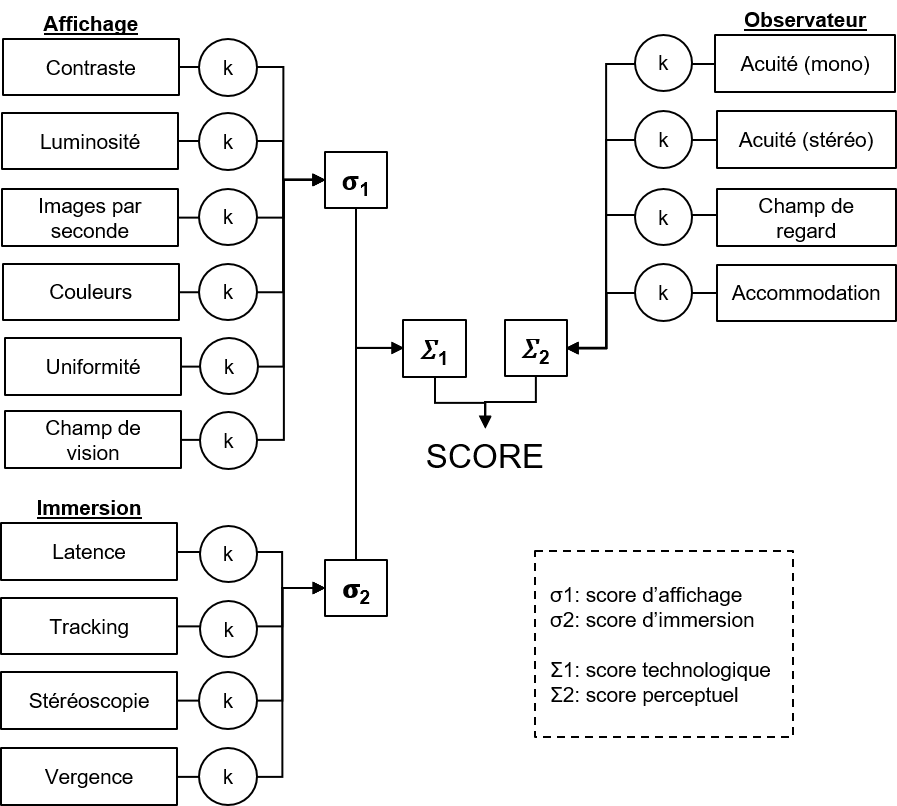
\includegraphics[scale=1]{Figures/Modele3_2}
		\caption{Troisième modélisation du score de réalisme.}
		\label{fig:modèle_3}
	\end{figure}
	
	\section{Modèle définitif}		
	\par En définitive, après un certain nombre d'itérations, de reconstructions, de nouvelles réflexions et de correction -notamment grâce à l'avis de reviewers des publications qui présentent ce modèle de score- on parvient à une version que l'on estime satisfaisante.
	
	\par On propose un modèle de score divisé en douze critères distribués en deux sections: une partie indices de vision et une partie indices d'immersion. La division des critères est faite telle que la première partie représente les informations qu'un œil recevrait à l'intérieur d'un simulateur tandis que la deuxième catégorie concerne ce que le système immersif offre à l'utilisateur pour participer à l'immersion. L'immersion est évidemment également réalisée via d'autres processus et nous avons seulement couvert les indices liés au hardware. Les critères sont répertoriés comme suit. Une vue d'ensemble du modèle est présentée Fig. \ref{fig:modèle_définitif}.
	
	\begin{itemize}\itemsep12pt
		\item \textbf{Indices de vision:} contraste et luminosité (luminance), images par seconde, nombre de couleurs affichables, champ de vision, acuités monoscopique et stéréoscopique.
		\item \textbf{Indices d'immersion:} latence, champ de regard, stéréoscopie, tracking, uniformité et convergence des caméras (laquelle est directement liée au mouvement des yeux).
	\end{itemize}
	
	\par Les critères de luminance et de contraste sont fusionnés. De par la nature du contraste (un ratio de luminances) ces deux critères semblent indissociables. Le critère de vergence est simplement renommé en <<~convergence des caméras~>> car il portait à confusion. Le critère <<~Accommodation~>> qui jugeait de la présence ou non du conflit accommodation-vergence n'était pas pertinent car il n'existe aujourd'hui aucun système de VR déployé industriellement\footnote{Pour voir la liste des systèmes sans conflit accommodation-vergence, se rapporter à \citep{mehrabi_making_2013}.} permettant de visualiser des images en 3D sans générer ce type de conflit ; il a donc été supprimé.
	
	\par La plus grosse modification reste le passage en deux catégories contre trois dans la précédente modélisation. La catégorie observateur portait à confusion, regroupait des critères qui avaient toute légitimité pour être dans les deux autres catégories. Les critères (moins le critère Accommodation, supprimé) ont donc été redistribués dans leur catégorie légitime. Celles ci sont en plus renommées de manière plus pertinente, pour correspondre plutôt au système, que l'on cherche à évaluer, et non à la vision humaine (sur laquelle on se base).
	
	\par Maintenant que nous avons défini comment le modèle se construisait, il convient de rentrer plus avant dans le détail et de présenter les critères retenus, un par un. A l'image des différentes modélisations du score, on déroulera rapidement les étapes de notation quand elles existent.
	
	\begin{figure}[h]
		\centering
		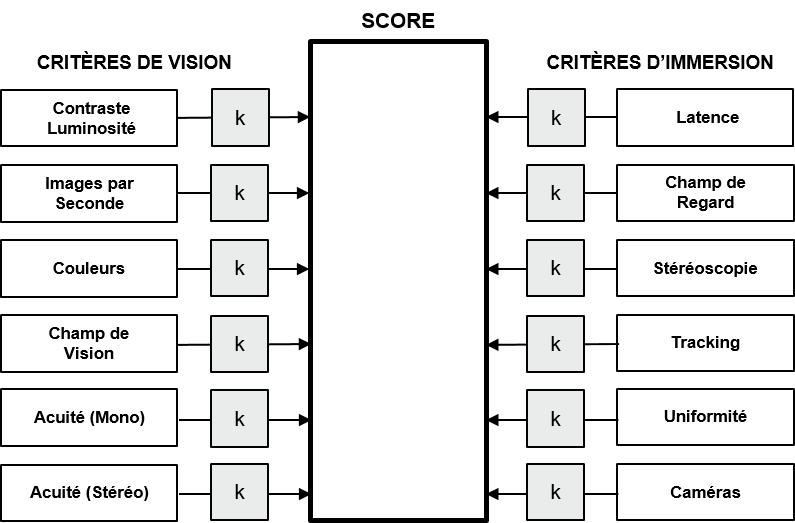
\includegraphics[scale=1.1]{Figures/ModeleDefinitif_2}
		\caption{Dernière modélisation du score de réalisme.}
		\label{fig:modèle_définitif}
	\end{figure}